\begin{figure} [H]
	\begin{center}
		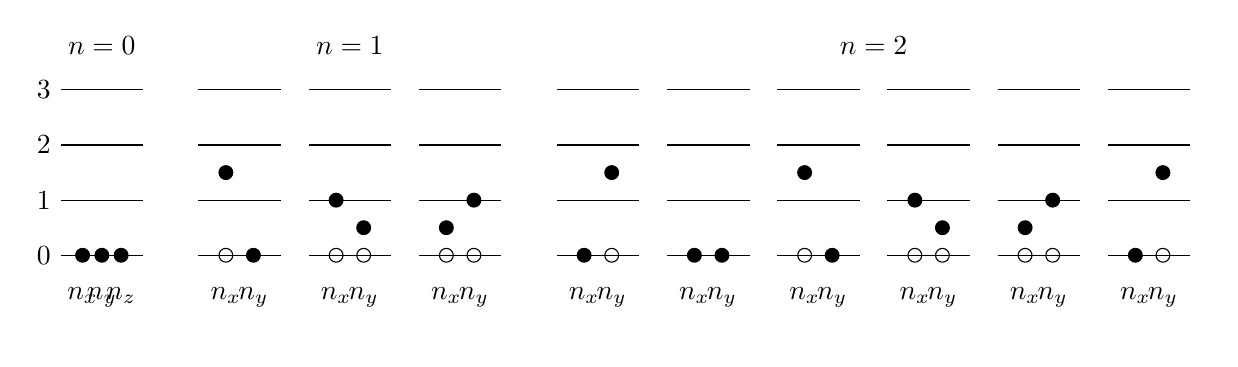
\begin{tikzpicture}[scale=0.35]
		\begin{scope}
		\foreach \i in {0,...,3}
		{
			\draw (-1,2*\i) node[anchor=east] {$\i$} --(2,2*\i);
		}
		\filldraw (-0.2,0) node[anchor=north,inner sep=.4cm] {$n_x$} circle (0.25cm); 
		\filldraw (0.5,0) node[anchor=north,inner sep=.4cm] {$n_y$} circle (0.25cm);
		\filldraw (1.2,0) node[anchor=north,inner sep=.4cm] {$n_z$} circle (0.25cm);
		\node[] at (0.5,7.6) {$n=0$};
		\end{scope}
		\begin{scope}[xshift=5cm]
		\foreach \i in {0,...,3}
		{
			\draw (-1,2*\i) --(2,2*\i);
		}
		\draw (0,0) node[anchor=north,inner sep=.4cm] {$n_x$} circle (0.25cm); 
		\filldraw (1,0) node[anchor=north,inner sep=.4cm] {$n_y$} circle (0.25cm);
		\filldraw (0,3) circle (0.25cm);
		\end{scope}
		\begin{scope}[xshift=9cm]
		\foreach \i in {0,...,3}
		{
			\draw (-1,2*\i) --(2,2*\i);
		}
		\draw (0,0) node[anchor=north,inner sep=.4cm] {$n_x$} circle (0.25cm); 
		\draw (1,0) node[anchor=north,inner sep=.4cm] {$n_y$} circle (0.25cm);
		\filldraw (0,2) circle (0.25cm); 
		\filldraw (1,1) circle (0.25cm); 
		\node[] at (0.5,7.6) {$n=1$};
		\end{scope}
		\begin{scope}[xshift=13cm]
		\foreach \i in {0,...,3}
		{
			\draw (-1,2*\i) --(2,2*\i);
		}
		\draw (0,0) node[anchor=north,inner sep=.4cm] {$n_x$} circle (0.25cm); 
		\draw (1,0) node[anchor=north,inner sep=.4cm] {$n_y$} circle (0.25cm);
		\filldraw (0,1) circle (0.25cm); 
		\filldraw (1,2) circle (0.25cm); 
		\end{scope}
		\begin{scope}[xshift=18cm]
		\foreach \i in {0,...,3}
		{
			\draw (-1,2*\i) --(2,2*\i);
		}
		\filldraw (0,0) node[anchor=north,inner sep=.4cm] {$n_x$} circle (0.25cm); 
		\draw (1,0) node[anchor=north,inner sep=.4cm] {$n_y$} circle (0.25cm);
		\filldraw (1,3) circle (0.25cm); 
		\end{scope}
		\begin{scope}[xshift=22cm]
		\foreach \i in {0,...,3}
		{
			\draw (-1,2*\i) --(2,2*\i);
		}
		\filldraw (0,0) node[anchor=north,inner sep=.4cm] {$n_x$} circle (0.25cm); 
		\filldraw (1,0) node[anchor=north,inner sep=.4cm] {$n_y$} circle (0.25cm);
		\end{scope}
		\begin{scope}[xshift=26cm]
		\foreach \i in {0,...,3}
		{
			\draw (-1,2*\i) --(2,2*\i);
		}
		\draw (0,0) node[anchor=north,inner sep=.4cm] {$n_x$} circle (0.25cm); 
		\filldraw (1,0) node[anchor=north,inner sep=.4cm] {$n_y$} circle (0.25cm);
		\filldraw (0,3) circle (0.25cm);
		\node[] at (2.5,7.6) {$n=2$};
		\end{scope}
		\begin{scope}[xshift=30cm]
		\foreach \i in {0,...,3}
		{
			\draw (-1,2*\i) --(2,2*\i);
		}
		\draw (0,0) node[anchor=north,inner sep=.4cm] {$n_x$} circle (0.25cm); 
		\draw (1,0) node[anchor=north,inner sep=.4cm] {$n_y$} circle (0.25cm);
		\filldraw (0,2) circle (0.25cm); 
		\filldraw (1,1) circle (0.25cm); 
		\end{scope}
		\begin{scope}[xshift=34cm]
		\foreach \i in {0,...,3}
		{
			\draw (-1,2*\i) --(2,2*\i);
		}
		\draw (0,0) node[anchor=north,inner sep=.4cm] {$n_x$} circle (0.25cm); 
		\draw (1,0) node[anchor=north,inner sep=.4cm] {$n_y$} circle (0.25cm);
		\filldraw (0,1) circle (0.25cm); 
		\filldraw (1,2) circle (0.25cm); 
		\end{scope}
		\begin{scope}[xshift=38cm]
		\foreach \i in {0,...,3}
		{
			\draw (-1,2*\i) --(2,2*\i);
		}
		\filldraw (0,0) node[anchor=north,inner sep=.4cm] {$n_x$} circle (0.25cm); 
		\draw (1,0) node[anchor=north,inner sep=.4cm] {$n_y$} circle (0.25cm);
		\filldraw (1,3) circle (0.25cm); 
		\end{scope}
		\end{tikzpicture}
	\end{center}

	\begin{center}
		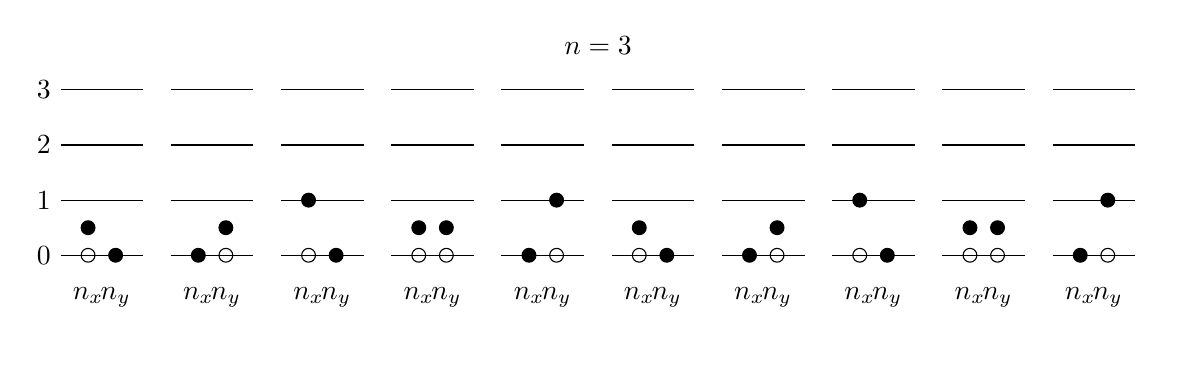
\begin{tikzpicture}[scale=0.35]
		\begin{scope}
		\foreach \i in {0,...,3}
		{
			\draw (-1,2*\i) node[anchor=east] {$\i$} --(2,2*\i);
		}
		\draw (0,0) node[anchor=north,inner sep=.4cm] {$n_x$} circle (0.25cm); 
		\filldraw (1,0) node[anchor=north,inner sep=.4cm] {$n_y$} circle (0.25cm);
		\filldraw (0,1) circle (0.25cm);
		\end{scope}
		\begin{scope}[xshift=4cm]
		\foreach \i in {0,...,3}
		{
			\draw (-1,2*\i) --(2,2*\i);
		}
		\filldraw (0,0) node[anchor=north,inner sep=.4cm] {$n_x$} circle (0.25cm); 
		\draw (1,0) node[anchor=north,inner sep=.4cm] {$n_y$} circle (0.25cm);
		\filldraw (1,1) circle (0.25cm); 
		\end{scope}
		\begin{scope}[xshift=8cm]
		\foreach \i in {0,...,3}
		{
			\draw (-1,2*\i) --(2,2*\i);
		}
		\draw (0,0) node[anchor=north,inner sep=.4cm] {$n_x$} circle (0.25cm); 
		\filldraw (1,0) node[anchor=north,inner sep=.4cm] {$n_y$} circle (0.25cm);
		\filldraw (0,2) circle (0.25cm);
		\end{scope}
		\begin{scope}[xshift=12cm]
		\foreach \i in {0,...,3}
		{
			\draw (-1,2*\i) --(2,2*\i);
		}
		\draw (0,0) node[anchor=north,inner sep=.4cm] {$n_x$} circle (0.25cm); 
		\draw (1,0) node[anchor=north,inner sep=.4cm] {$n_y$} circle (0.25cm);
		\filldraw (0,1) circle (0.25cm); 
		\filldraw (1,1) circle (0.25cm);
		\end{scope}
		\begin{scope}[xshift=16cm]
		\foreach \i in {0,...,3}
		{
			\draw (-1,2*\i) --(2,2*\i);
		}
		\filldraw (0,0) node[anchor=north,inner sep=.4cm] {$n_x$} circle (0.25cm); 
		\draw (1,0) node[anchor=north,inner sep=.4cm] {$n_y$} circle (0.25cm); 
		\filldraw (1,2) circle (0.25cm);
		\node[] at (2.5,7.6) {$n=3$};
		\end{scope}
		\begin{scope}[xshift=20cm]
		\foreach \i in {0,...,3}
		{
			\draw (-1,2*\i) --(2,2*\i);
		}
		\draw (0,0) node[anchor=north,inner sep=.4cm] {$n_x$} circle (0.25cm); 
		\filldraw (1,0) node[anchor=north,inner sep=.4cm] {$n_y$} circle (0.25cm);
		\filldraw (0,1) circle (0.25cm);
		\end{scope}
		\begin{scope}[xshift=24cm]
		\foreach \i in {0,...,3}
		{
			\draw (-1,2*\i) --(2,2*\i);
		}
		\filldraw (0,0) node[anchor=north,inner sep=.4cm] {$n_x$} circle (0.25cm); 
		\draw (1,0) node[anchor=north,inner sep=.4cm] {$n_y$} circle (0.25cm);
		\filldraw (1,1) circle (0.25cm); 
		\end{scope}
		\begin{scope}[xshift=28cm]
		\foreach \i in {0,...,3}
		{
			\draw (-1,2*\i) --(2,2*\i);
		}
		\draw (0,0) node[anchor=north,inner sep=.4cm] {$n_x$} circle (0.25cm); 
		\filldraw (1,0) node[anchor=north,inner sep=.4cm] {$n_y$} circle (0.25cm);
		\filldraw (0,2) circle (0.25cm);
		\end{scope}
		\begin{scope}[xshift=32cm]
		\foreach \i in {0,...,3}
		{
			\draw (-1,2*\i) --(2,2*\i);
		}
		\draw (0,0) node[anchor=north,inner sep=.4cm] {$n_x$} circle (0.25cm); 
		\draw (1,0) node[anchor=north,inner sep=.4cm] {$n_y$} circle (0.25cm);
		\filldraw (0,1) circle (0.25cm); 
		\filldraw (1,1) circle (0.25cm);
		\end{scope}
		\begin{scope}[xshift=36cm]
		\foreach \i in {0,...,3}
		{
			\draw (-1,2*\i) --(2,2*\i);
		}
		\filldraw (0,0) node[anchor=north,inner sep=.4cm] {$n_x$} circle (0.25cm); 
		\draw (1,0) node[anchor=north,inner sep=.4cm] {$n_y$} circle (0.25cm); 
		\filldraw (1,2) circle (0.25cm);
		\end{scope}
		\end{tikzpicture}
	\end{center}
	\caption{Possible states of a three dimensional harmonic oscillator.}
	\label{fig:schematic_3d}
\end{figure}